\chapter{Implementazione}
\label{chp:implementazione_nuovo}

Questo capitolo descrive l'implementazione del sistema sperimentale sviluppato
per confrontare algoritmi di stima della cardinalità su flussi (\emph{stream})
e per studiare le loro proprietà in modalità di flusso e di fusione
(\emph{merge}). Il capitolo è costruito
attorno a tre nuclei principali:
\begin{itemize}
    \item gli algoritmi, la loro interfaccia comune e le scelte adottate per
    tradurre in codice le strutture descritte nella letteratura;
    \item le funzioni di hash, il loro ruolo nella semantica delle strutture
    di riassunto (\emph{sketch}) e la
    ragione della loro selezione;
    \item l'infrastruttura di valutazione (\emph{framework}), cioè il modo in
    cui dataset, algoritmi,
    metriche e serializzazione dei risultati sono stati composti in un'unica
    catena di esecuzione (\emph{pipeline}) riproducibile.
\end{itemize}

Il nucleo del sistema è implementato in \texttt{C++}, mentre in \texttt{Python}
sono stati sviluppati il generatore del dataset sintetico usato nella tesi e
gli script di orchestrazione batch degli esperimenti.

\section{Obiettivi progettuali}

L'implementazione non nasce come semplice raccolta di algoritmi isolati, ma
come piattaforma di confronto. Di conseguenza il progetto è stato guidato da
quattro obiettivi principali.

Il primo obiettivo è uniformare algoritmi diversi sotto un contratto comune.
Probabilistic Counting, LogLog, HyperLogLog e HyperLogLog++ condividono infatti
la stessa interfaccia astratta, pur avendo stati interni e regole di stima
molto differenti. Questa scelta permette al resto del sistema di invocare gli
algoritmi senza conoscere i dettagli delle singole implementazioni.

Il secondo obiettivo è separare chiaramente la responsabilità dello sketch dalla
responsabilità dell'hashing. In tutti gli algoritmi basati su registri, la
funzione di hash non è un dettaglio accessorio, ma parte della semantica del
calcolo. Per questo motivo l'hash non è codificato rigidamente dentro ciascun
algoritmo, ma viene iniettato tramite un'interfaccia comune.

Il terzo obiettivo è rendere l'infrastruttura sperimentale riproducibile. Il
seed, i parametri degli algoritmi, il dataset, la modalità di esecuzione e il
percorso del file dei risultati devono essere tracciabili in modo deterministico
e coerente tra esecuzione interattiva, orchestrazione batch e analisi finale.

Il quarto obiettivo è mantenere separati il livello algoritmico e il livello di
misura. Il codice che aggiorna uno sketch non deve dipendere dal formato del
dataset, dalla pianificazione dei punti di controllo (\emph{checkpoint}) o
dalla serializzazione in file
\texttt{CSV}. Questa separazione riduce il rischio di introdurre dipendenze
accidentali e rende l'infrastruttura estendibile a nuove famiglie di algoritmi e a
nuovi esperimenti.

\section{Architettura generale del sistema}

L'architettura complessiva è organizzata in tre strati:
\begin{itemize}
    \item uno strato algoritmico, che contiene le implementazioni concrete degli
    sketch e il catalogo degli identificatori canonici;
    \item uno strato di supporto, che comprende dataset binario, funzioni di
    hash e tipi di configurazione;
    \item uno strato di coordinamento sperimentale, che comprende la riga di
    comando, il framework di valutazione, la raccolta delle metriche e la
    scrittura dei risultati.
\end{itemize}

Questa scomposizione corrisponde direttamente alla struttura del repository:
\codepath{algorithms/} per gli sketch,
\codepath{hashing/} per le funzioni di hash,
\codepath{dataset/} per il formato binario,
\codepath{simulation/} per il protocollo di valutazione e
\codepath{cli/} per il coordinamento dell'esecuzione.

La Figura~\ref{fig:system-architecture} riassume i moduli principali, il verso
di utilizzo tra di essi e il rapporto con gli strumenti esterni in
\texttt{Python}.

\clearpage
\begin{landscape}
    \begin{figure}[p]
        \centering
        \resizebox{0.98\linewidth}{!}{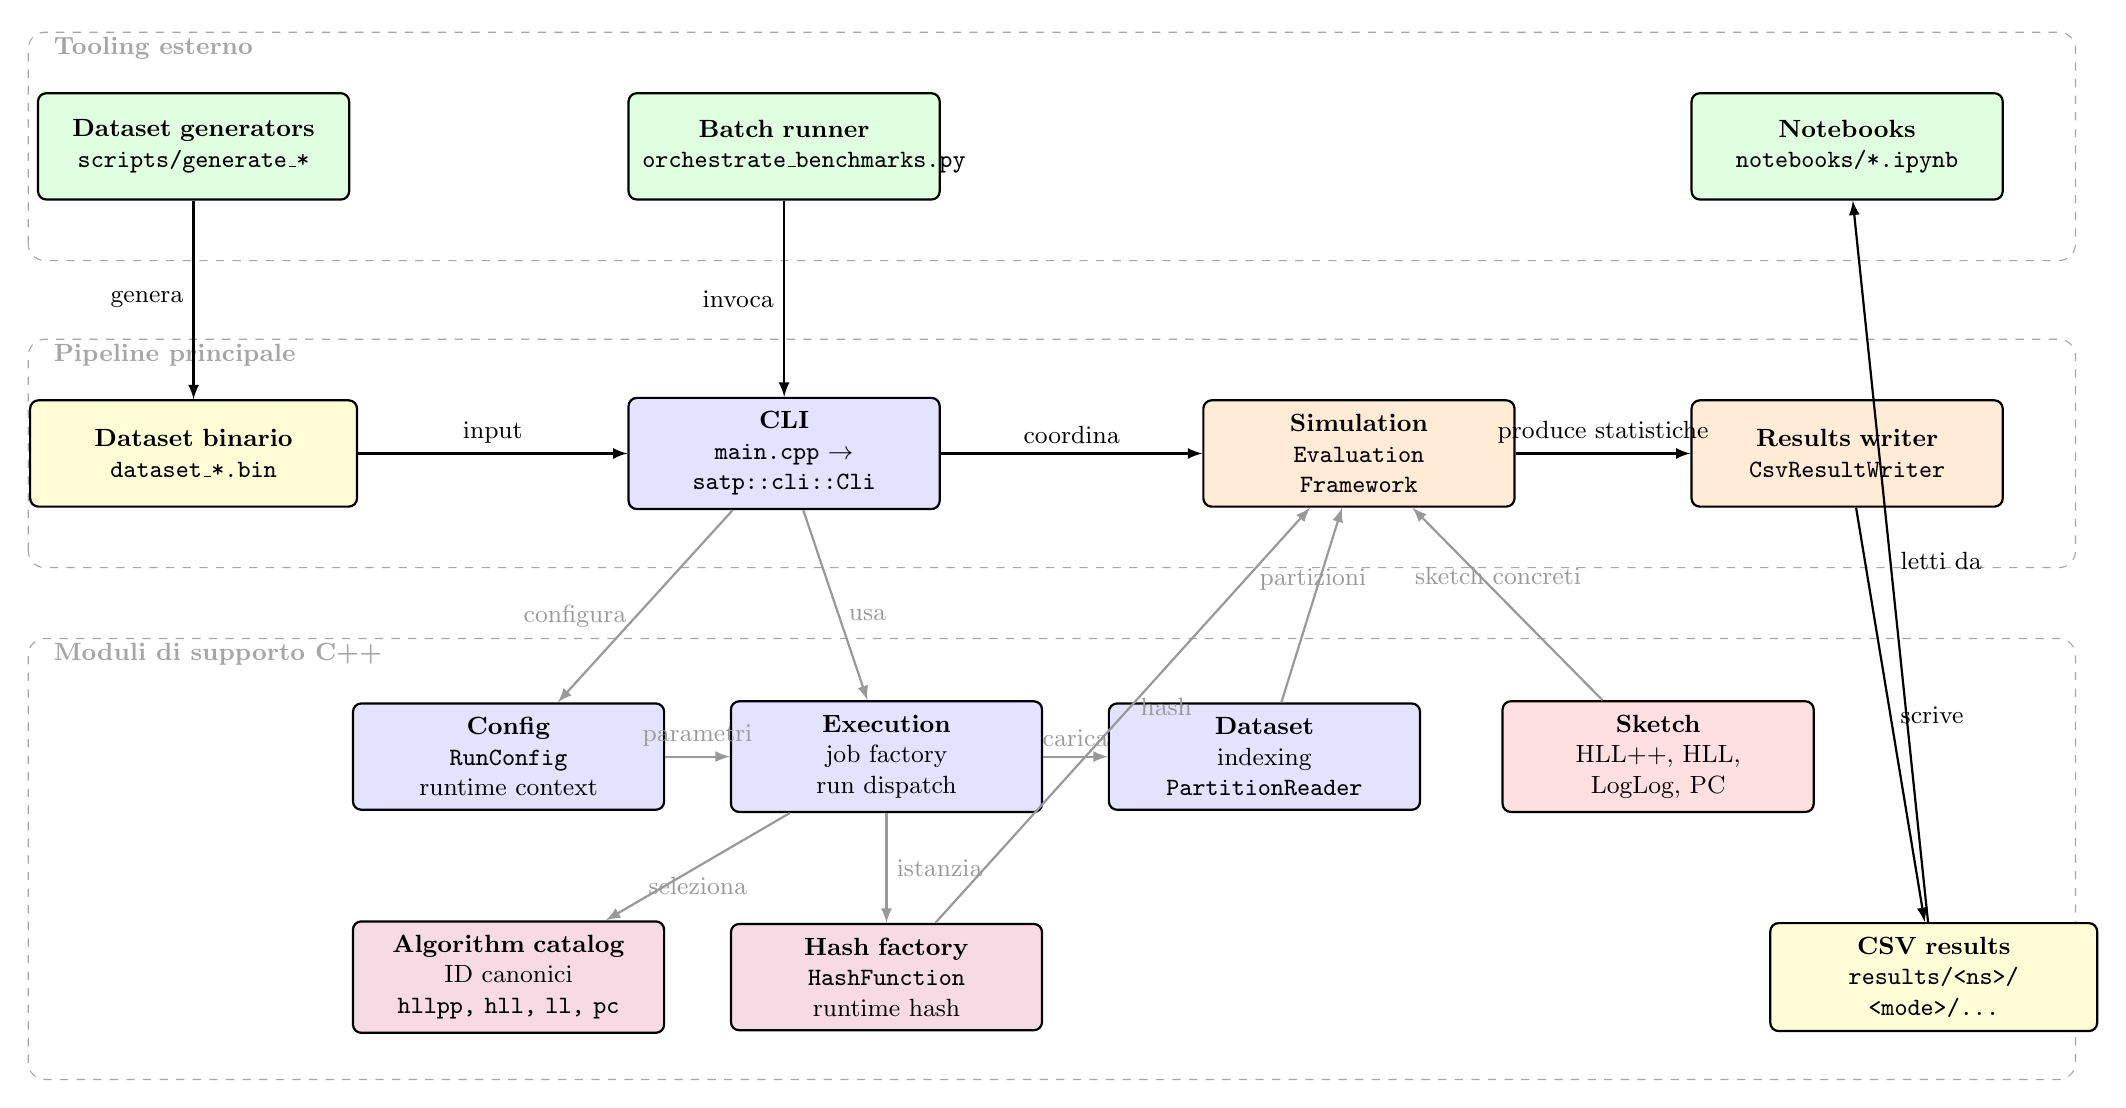
\begin{tikzpicture}[x=1cm,y=1cm,>=latex,font=\small]
    \tikzstyle{module}=[draw, rounded corners=3pt, thick, align=center,
        text width=3.6cm, minimum height=1.35cm, inner sep=5pt]
    \tikzstyle{artifact}=[draw, rounded corners=3pt, thick, align=center,
        text width=3.8cm, minimum height=1.35cm, inner sep=5pt]
    \tikzstyle{flow}=[->, thick]
    \tikzstyle{support}=[->, thick, gray!80]

    % Layer frames
    \draw[dashed, rounded corners=6pt, gray!70] (-2.1,7.3) rectangle (23.9,10.2);
    \node[anchor=west, gray!70] at (-1.9,10.0) {\textbf{Tooling esterno}};

    \draw[dashed, rounded corners=6pt, gray!70] (-2.1,3.4) rectangle (23.9,6.3);
    \node[anchor=west, gray!70] at (-1.9,6.1) {\textbf{Pipeline principale}};

    \draw[dashed, rounded corners=6pt, gray!70] (-2.1,-3.1) rectangle (23.9,2.5);
    \node[anchor=west, gray!70] at (-1.9,2.3) {\textbf{Moduli di supporto C++}};

    % External tooling
    \node[module, fill=green!12] (generators) at (0.0,8.75)
        {\textbf{Dataset generators}\\\texttt{scripts/generate\_*}};
    \node[module, fill=green!12] (orchestrator) at (7.5,8.75)
        {\textbf{Batch runner}\\\texttt{orchestrate\_benchmarks.py}};
    \node[module, fill=green!12] (notebooks) at (21.0,8.75)
        {\textbf{Notebooks}\\\texttt{notebooks/*.ipynb}};

    % Main pipeline
    \node[artifact, fill=yellow!16] (datasetfile) at (0.0,4.85)
        {\textbf{Dataset binario}\\\texttt{dataset\_*.bin}};
    \node[module, fill=blue!11] (cli) at (7.5,4.85)
        {\textbf{CLI}\\\texttt{main.cpp} $\rightarrow$ \texttt{satp::cli::Cli}};
    \node[module, fill=orange!16] (simulation) at (14.8,4.85)
        {\textbf{Simulation}\\\texttt{Evaluation}\\\texttt{Framework}};
    \node[module, fill=orange!16] (writer) at (21.0,4.85)
        {\textbf{Results writer}\\\texttt{CsvResultWriter}};

    % Support modules
    \node[module, fill=blue!11] (config) at (4.0,1.0)
        {\textbf{Config}\\\texttt{RunConfig}\\runtime context};
    \node[module, fill=blue!11] (execution) at (8.8,1.0)
        {\textbf{Execution}\\job factory\\run dispatch};
    \node[module, fill=blue!11] (dataset) at (13.6,1.0)
        {\textbf{Dataset}\\indexing\\\texttt{PartitionReader}};
    \node[module, fill=purple!14] (hashing) at (8.8,-1.8)
        {\textbf{Hash factory}\\\texttt{HashFunction}\\runtime hash};
    \node[module, fill=purple!14] (catalog) at (4.0,-1.8)
        {\textbf{Algorithm catalog}\\ID canonici\\\texttt{hllpp, hll, ll, pc}};
    \node[module, fill=red!12] (algorithms) at (18.6,1.0)
        {\textbf{Sketch}\\HLL++, HLL,\\LogLog, PC};
    \node[artifact, fill=yellow!16] (results) at (22.1,-1.8)
        {\textbf{CSV results}\\\texttt{results/<ns>/}\\\texttt{<mode>/...}};

    % Main flow
    \draw[flow] (generators) -- node[left, pos=0.5] {genera} (datasetfile);
    \draw[flow] (orchestrator) -- node[left, pos=0.5] {invoca} (cli);
    \draw[flow] (datasetfile) -- node[above, pos=0.5] {input} (cli);
    \draw[flow] (cli) -- node[above, pos=0.5] {coordina} (simulation);
    \draw[flow] (simulation) -- node[above, pos=0.5] {produce statistiche} (writer);
    \draw[flow] (writer) -- node[right, pos=0.5] {scrive} (results);
    \draw[flow] (results) -- node[right, pos=0.5] {letti da} (notebooks);

    % Support relations
    \draw[support] (cli) -- node[left, pos=0.55] {configura} (config);
    \draw[support] (cli) -- node[right, pos=0.55] {usa} (execution);
    \draw[support] (config) -- node[above, pos=0.5] {parametri} (execution);
    \draw[support] (execution) -- node[above, pos=0.5] {carica} (dataset);
    \draw[support] (execution) -- node[right, pos=0.5] {istanzia} (hashing);
    \draw[support] (execution) -- node[below, pos=0.5] {seleziona} (catalog);
    \draw[support] (dataset) -- node[above, pos=0.52] {partizioni} (simulation);
    \draw[support] (hashing) -- node[right, pos=0.52] {hash} (simulation);
    \draw[support] (algorithms) -- node[above, pos=0.55] {sketch concreti} (simulation);
\end{tikzpicture}
}
        \caption{Architettura del sistema e principali dipendenze tra moduli e artefatti. Le frecce indicano chi usa chi oppure il verso del flusso dati}
        \label{fig:system-architecture}
    \end{figure}
\end{landscape}
\clearpage

Dal punto di vista operativo, la catena di esecuzione completa è la seguente:
\begin{enumerate}
    \item il dataset sintetico viene generato in \texttt{Python} e serializzato
    nel formato binario compresso usato dal framework;
    \item la riga di comando carica il dataset, ne legge i metadati e costruisce
    il contesto di esecuzione;
    \item il coordinatore di esecuzione seleziona gli algoritmi richiesti,
    istanzia la funzione di hash a tempo di esecuzione (\emph{runtime}) e
    prepara i descrittori dell'esperimento;
    \item il framework di valutazione percorre le partizioni del dataset e
    calcola le metriche in memoria;
    \item il modulo di scrittura dei risultati serializza le statistiche in file
    \texttt{CSV}, che vengono poi elaborati nei notebook del capitolo
    sperimentale.
\end{enumerate}

Questa architettura privilegia la separazione delle responsabilità. La riga di
comando conosce i parametri della sessione, ma non la logica interna degli
algoritmi. Gli algoritmi conoscono la propria logica di aggiornamento, ma non il
formato del dataset. Il framework di valutazione conosce il protocollo
sperimentale, ma non incorpora direttamente le politiche di generazione dei
grafici o la struttura dei notebook.

\section{Algoritmi di sketching}

\subsection{Criteri di scelta degli algoritmi}

Il nucleo algoritmico del progetto è dedicato al problema della stima del numero
di elementi distinti. Le implementazioni presenti seguono una progressione
storica e metodologica coerente con la letteratura studiata nei capitoli
precedenti.

La prima implementazione è \texttt{NaiveCounting}, usata come riferimento esatto
interno. Questa classe non viene esposta come algoritmo degli esperimenti
principali, ma è essenziale nei test del framework perché fornisce un
riferimento privo di errore di stima.

La seconda famiglia è \texttt{ProbabilisticCounting}, che deriva dal lavoro di
Flajolet e Martin \cite{Flajolet_Martin_1985}. Questa implementazione è
interessante perché rappresenta il primo punto della linea evolutiva degli
algoritmi probabilistici per il conteggio dei distinti.

La terza famiglia comprende \texttt{LogLog} e \texttt{HyperLogLog}, che
discendono rispettivamente dai lavori di Durand e Flajolet
\cite{Durand_Flajolet_2003} e di Flajolet, Fusy, Gandouet e Meunier
\cite{Flajolet_Fusy_Gandouet_Meunier_2007}. Questi due algoritmi condividono la
struttura a registri e consentono di studiare in modo diretto come varia la
qualità della stima a parità di idea architetturale di base.

L'ultima implementazione è \texttt{HyperLogLog++}, che segue la variante pratica
proposta da Heule, Nunkesser e Hall \cite{Heule_Nunkesser_Hall_2013}. È
l'algoritmo più importante della base di codice perché rappresenta sia il riferimento
per i confronti in modalità di flusso sia il punto di partenza per lo studio del
merge eterogeneo.

La selezione degli algoritmi non è quindi casuale. Essa copre:
\begin{itemize}
    \item un riferimento esatto;
    \item un primo algoritmo probabilistico compatto;
    \item due algoritmi a registri della famiglia LogLog e HyperLogLog;
    \item la variante più pratica e completa della stessa linea evolutiva.
\end{itemize}

Dal punto di vista del catalogo applicativo, gli esperimenti pubblici
espongono quattro identificatori canonici:
\texttt{hllpp}, \texttt{hll}, \texttt{ll}, \texttt{pc}. Nel file
\codepath{AlgorithmCatalog.cpp} è presente anche l'identificatore \texttt{naive}
per il riferimento interno, ma questo non fa parte dell'elenco pubblico degli
algoritmi selezionabili dalla riga di comando. In modo coerente,
\codepath{getIdsOfSupportedAlgorithms()} espone solo i quattro identificatori
pubblici e non include \texttt{naive}.

\subsection{Interfaccia comune}

L'interfaccia astratta comune è definita in
\codepath{Algorithm.h}. Ogni algoritmo riceve nel
costruttore un riferimento costante a una funzione di hash e deve implementare i
seguenti metodi:
\begin{itemize}
    \item \texttt{process(uint32\_t id)}, che aggiorna lo sketch con un nuovo
    valore;
    \item \texttt{count()}, che restituisce il conteggio esatto o la stima
    corrente;
    \item \texttt{merge(const Algorithm\& other)}, che combina due stati
    compatibili;
    \item \texttt{reset()}, che azzera lo stato interno;
    \item \texttt{getName()}, che restituisce il nome canonico usato nel resto
    del sistema.
\end{itemize}

Questa interfaccia esprime due scelte progettuali precise. La prima è che la
funzione di hash appartenga al contesto dell'algoritmo e non sia lasciata come
responsabilità del chiamante a ogni aggiornamento. La seconda è che il merge sia
parte dell'interfaccia di primo livello e non un'estensione opzionale aggiunta
solo ad alcuni algoritmi.

Nel framework esiste anche un controllo di concetto a livello di compilazione,
definito in \codepath{SketchFactory.h}, che
impedisce di usare nelle modalità di merge algoritmi privi dell'operazione di
fusione richiesta.

\subsection{Scelte progettuali comuni}

Pur seguendo lavori diversi, le implementazioni condividono alcune convenzioni.

La prima convenzione è la validazione esplicita dei parametri nel costruttore.
I limiti di \texttt{ProbabilisticCounting}, \texttt{LogLog},
\texttt{HyperLogLog} e \texttt{HyperLogLog++} non sono lasciati a vincoli
impliciti, ma producono eccezioni \texttt{invalid\_argument} se la
configurazione non appartiene al dominio supportato.

La seconda convenzione è la distinzione tra interfaccia astratta e overload
tipizzato del merge. Ogni classe implementa \texttt{merge(const Algorithm\&)}
con un controllo dinamico del tipo e poi delega a una variante tipizzata
\texttt{merge(const TipoConcreto\&)}. In questo modo il contratto comune resta
stabile, ma l'implementazione concreta può esprimere in modo chiaro i controlli
di compatibilità parametrica.

La terza convenzione è l'uso di identificatori canonici separati dal nome
stampato. Il catalogo algoritmico centralizza infatti la traduzione tra
identificatori brevi, usati dalla riga di comando e dai percorsi dei risultati,
e nomi completi, usati nei file \texttt{CSV} e nella tesi.

La quarta convenzione è la separazione tra stato interno dello sketch e logica
di serializzazione dei parametri. Il formato testuale dei parametri
\texttt{k=...}, \texttt{L=...} o combinazioni analoghe non è costruito dentro le
classi degli algoritmi, ma nel livello di coordinamento delle unità di
esecuzione (\emph{job}). Questo rende
più semplice mantenere coerenti descrizione testuale, nomi dei file dei
risultati e ricostruzione degli esperimenti.

\subsection{Implementazione dei singoli algoritmi}

\paragraph{Baseline esatta}
\texttt{NaiveCounting} mantiene un insieme ordinato di identificatori distinti
tramite \texttt{std::set<uint32\_t>}. Il metodo \texttt{process} inserisce un
elemento solo se non è già presente, il metodo \texttt{count} restituisce la
cardinalità dell'insieme e il merge esegue un'unione insiemistica. Questa classe
riceve comunque una funzione di hash, per uniformità di interfaccia, ma non la
usa nella logica interna.

\paragraph{Probabilistic Counting}
L'implementazione di \texttt{ProbabilisticCounting} segue l'idea originale di
Flajolet e Martin \cite{Flajolet_Martin_1985}. Lo stato è rappresentato da una
bitmap memorizzata in un intero a 32 bit, con il vincolo applicativo
\(L \in [1,31]\) e l'aggiornamento usa \texttt{hash32}, tronca il risultato a
\(L\) bit, individua la posizione del primo uno a partire dal bit meno
significativo con \texttt{countr\_zero} e attiva il bit corrispondente. La stima
usa invece \texttt{countr\_one} per ricavare l'indice del primo zero e applica
la costante di correzione \(\phi\) del metodo originario. Il merge usa
l'operatore OR bit per bit e richiede uguaglianza del parametro \(L\) nei due
sketch.

\paragraph{LogLog}
\texttt{LogLog} usa un vettore di registri \texttt{uint8\_t} e mantiene in modo
incrementale la somma dei registri nella quantità \(\sum_j M[j]\) aggiornata a
ogni inserimento. Questa scelta evita di ricalcolare l'intera somma a ogni
chiamata di \texttt{count}. Il costruttore impone un'implementazione aderente
al dominio usato nel lavoro di riferimento. Nel dominio implementato, con
\(k \in [4,16]\) e \(L = 32\) l'aggiornamento estrae i primi \(k\) bit
dell'hash a 32 bit per selezionare il registro e usa il resto dei bit per
calcolare il rango \(\rho\) e il merge
applica il massimo componente per componente e poi ricostruisce la somma dei
registri aggiornata.

\paragraph{HyperLogLog}
\texttt{HyperLogLog} mantiene ancora un vettore di registri \texttt{uint8\_t},
ma a differenza di \texttt{LogLog} memorizza anche due quantità aggregate che
servono direttamente alla stima: la somma delle potenze inverse
\(\sum_j 2^{-M[j]}\) e il numero di registri nulli. Questa scelta rende più
efficiente la valutazione dei diversi regimi di stima. Anche qui il dominio è
ristretto al caso classico. Nel dominio implementato, con \(k \in [4,16]\) e
\(L = 32\) il metodo
\texttt{count} implementa tre regimi: correzione per cardinalità piccole tramite
\emph{linear counting}, stima armonica nel regime intermedio e correzione
logaritmica nel regime grande, in accordo con \cite{Flajolet_Fusy_Gandouet_Meunier_2007}.
Il merge richiede uguaglianza dei parametri \(k\) e \(L\) oltre al numero di
bucket e poi
ricalcola le grandezze aggregate sullo stato risultante.

\paragraph{HyperLogLog++}
\texttt{HyperLogLog++} è l'implementazione più articolata della base di codice.
Il parametro costruttivo è memorizzato come \(p\) ma nel resto del framework viene
serializzato uniformemente come \texttt{k=<valore>} per mantenere un formato dei
parametri coerente tra famiglie algoritmiche. Nel dominio supportato con
\(p \in [4,18]\) questa implementazione, a differenza di \texttt{HyperLogLog},
usa sempre l'hash a 64 bit.

Lo stato interno alterna due rappresentazioni:
\begin{itemize}
    \item una rappresentazione sparsa, basata su un insieme temporaneo
    \texttt{tmpSet} e su una lista compressa \texttt{sparseList};
    \item una rappresentazione densa, basata su un vettore di registri
    \texttt{registers}.
\end{itemize}

La transizione dalla forma sparsa alla forma densa avviene quando il costo in
bit della rappresentazione sparsa supera il costo della rappresentazione densa.
Questa scelta è implementata confrontando \texttt{compressedSparseBits()} e
\texttt{denseBits()}. La stima finale integra inoltre due componenti aggiuntive:
una tabella di bias e una soglia per la scelta tra \emph{linear counting} e
stima corretta, entrambe mantenute in \codepath{hllpp_tables.cpp}.

Il merge diretto è definito solo quando il parametro \(p\) coincide nei due
sketch. Se entrambi gli sketch sono ancora in formato sparso, il merge procede
fondendo le codifiche compresse; se almeno uno dei due è già in formato denso,
entrambi vengono prima portati in forma densa e poi fusi registro per registro.
La classe espone anche due operazioni aggiuntive, \texttt{reducedTo(...)} e
\texttt{reducedToNaive(...)}, usate nel framework di merge eterogeneo per
studiare il caso di mismatch di precisione. Nei casi \texttt{recoverable} di
mismatch di precisione, il framework costruisce sia il riferimento seriale sia
il riferimento omogeneo alla precisione minima \(\min(k_{left}, k_{right})\) in
modo coerente per entrambi i confronti.

\section{Funzioni di hash}

\subsection{Ruolo dell'hash negli sketch}

Negli algoritmi implementati l'hash non serve solo a ottenere un identificatore
apparente uniforme. Esso è parte integrante della semantica del metodo.

In \texttt{ProbabilisticCounting}, i bit dell'hash determinano la posizione del
primo uno osservato nella bitmap. In \texttt{LogLog} e \texttt{HyperLogLog}, i
primi \(k\) bit identificano il registro, mentre i bit restanti definiscono un
rango indicato con \(\rho\) e nel caso di \texttt{HyperLogLog++} la stessa idea
viene estesa al caso a 64 bit e viene riutilizzata sia nella rappresentazione
densa sia in quella sparsa.

Da questa osservazione discende una conseguenza importante per tutta la tesi: il
processo di fusione corretto non dipende soltanto dal tipo dell'algoritmo, ma anche dalla
semantica condivisa dell'hash. Due sketch costruiti con hash o seed diversi non
stanno necessariamente rappresentando gli stessi sottoflussi logici.

\subsection{Interfaccia comune delle hash}

L'astrazione comune delle funzioni di hash è definita in
\codepath{HashFunction.h}. L'interfaccia espone tre operazioni:
\begin{itemize}
    \item \texttt{hash64(uint64\_t)}, che rappresenta l'operazione fondamentale;
    \item \texttt{hash32(uint64\_t)}, che per default proietta il risultato a
    64 bit sui 32 bit più significativi;
    \item \texttt{name()}, che restituisce il nome canonico della funzione.
\end{itemize}

Questa interfaccia permette di iniettare una funzione di hash in qualunque
algoritmo senza cambiare il contratto della classe \texttt{Algorithm}. Il fatto
che \texttt{hash32} sia definito come proiezione standard della versione a
64 bit consente inoltre di mantenere un'unica gerarchia di hash anche quando
algoritmi diversi operano su ampiezze di parola diverse.

\subsection{Funzioni scelte e motivazione}

La selezione delle funzioni di hash è centralizzata in
\codepath{HashFactory.cpp}. Il sistema supporta quattro nomi
canonici:
\texttt{splitmix64}, \texttt{xxhash64}, \texttt{murmurhash3}, \texttt{siphash24}.

Questa scelta risponde a un criterio di copertura del dominio sperimentale,
piuttosto che alla ricerca di una singola funzione ottima in assoluto.

\texttt{splitmix64} è la funzione di default del sistema. È semplice da
istanziare, non richiede stato esterno nel costruttore corrente e fornisce un
riferimento leggero e deterministico per tutti gli esperimenti.

\texttt{xxhash64} rappresenta una funzione non crittografica molto diffusa nelle
applicazioni pratiche, con supporto esplicito al seed nella classe
\texttt{XXHash64}. La sua presenza è utile perché combina semplicità
implementativa e uso realistico nei sistemi applicativi.

\texttt{murmurhash3} rappresenta un secondo riferimento pratico molto diffuso.
Nel codice viene usata una variante ridotta a un blocco da 64 bit, seedata e
adatta al caso in cui gli identificatori siano interi a 32 bit promossi a 64
bit.

\texttt{siphash24} completa il quadro con una funzione della famiglia SipHash.
Nel codice attuale viene istanziata con le chiavi di default della classe
\texttt{SipHash24}. La sua presenza è utile perché aggiunge al confronto una
funzione con una costruzione diversa da quelle puramente non crittografiche più
comuni.

L'obiettivo della selezione non è quindi confrontare soltanto velocità diverse,
ma rendere possibile una matrice sperimentale in cui la semantica dell'hash può
essere mantenuta costante oppure modificata in modo controllato.

\subsection{Seed e riproducibilità}

Il seed entra nel sistema in due punti distinti. Il primo è il seed del dataset,
che viene memorizzato nell'header binario e propagato nel contesto runtime. Il
secondo è il seed locale della funzione di hash, che nel caso del merge
eterogeneo può essere impostato separatamente per lato sinistro e destro.

La factory \codepath{getHashFunctionBy(...)} applica le seguenti regole:
\begin{itemize}
    \item se non viene specificato alcun nome, viene istanziata
    \texttt{SplitMix64};
    \item se viene specificato un nome, la factory richiede anche un seed;
    \item \texttt{XXHash64} e \texttt{MurmurHash3} usano esplicitamente il seed
    passato;
    \item \texttt{SplitMix64} ignora il seed a livello della classe concreta;
    \item \texttt{SipHash24} è istanziata con le chiavi di default previste
    dalla classe concreta, quindi il seed configurato nella sessione non agisce
    come leva uniforme su questa hash.
\end{itemize}

Nel flusso standard della riga di comando, il seed usato per la funzione di hash
ha come fallback il seed del dataset. Nel merge eterogeneo, invece, i campi
\texttt{leftHashSeed} e \texttt{rightHashSeed} prevalgono quando sono
valorizzati, mentre in assenza di override resta attivo il fallback al seed del
dataset.

\section{Framework sperimentale}

\subsection{Requisiti del framework}

L'infrastruttura sperimentale doveva soddisfare contemporaneamente requisiti
diversi.

Dal lato algoritmico, doveva essere possibile usare lo stesso schema di
esecuzione per sketch differenti senza duplicare codice di attraversamento del
dataset.

Dal lato metodologico, dovevano essere supportate tre modalità diverse:
\begin{itemize}
    \item una modalità di flusso, per osservare l'evoluzione della stima lungo i
    prefissi;
    \item una modalità di fusione omogenea, per confrontare fusione e riferimento
    seriale;
    \item una modalità di fusione eterogenea, per descrivere casi validi,
    recuperabili o non validi e misurarne il comportamento.
\end{itemize}

Dal lato operativo, il sistema doveva derivare automaticamente dai metadati del
dataset il numero di partizioni, la dimensione della partizione e il seed, così
da evitare configurazioni incoerenti tra dataset e sessione di esecuzione.

\subsection{Struttura del framework}

La struttura pubblica è organizzata in tre coordinatori principali:
\begin{itemize}
    \item \codepath{satp::cli::Cli} come frontiera interattiva verso
    l'utente;
    \item il modulo pubblico del dataset, esposto da
    \codepath{Dataset.h}, come punto di accesso
    all'indicizzazione e al caricamento delle partizioni;
    \item \codepath{satp::evaluation::EvaluationFramework}, riesportato da
    \codepath{Simulation.h}, come coordinatore delle modalità
    di valutazione.
\end{itemize}

La classe \texttt{EvaluationFramework} contiene un indice del dataset binario,
un oggetto \texttt{EvaluationMetadata} derivato dai metadati del dataset e una
funzione di hash posseduta tramite \texttt{unique\_ptr}. Da questa struttura
discende una proprietà importante: il framework non ha bisogno di rileggere la
configurazione globale a ogni esecuzione, perché il suo contesto fondamentale è
già materializzato all'atto della costruzione.

Nel flusso eterogeneo, però, la funzione di hash posseduta da
\texttt{EvaluationFramework} non governa direttamente i due lati del confronto.
In \codepath{HeterogeneousMergeEvaluation.tpp}, per ogni coppia vengono
istanziate hash dedicate a partire dal descrittore:
hash sinistra, hash destra, hash del riferimento seriale e hash del riferimento
omogeneo quando presente. In termini operativi, le istanze vengono costruite per
ogni coppia con \codepath{getHashFunctionBy(...)} usando i campi
\texttt{left}, \texttt{right}, \texttt{serialReference} e
\texttt{homogeneousBaseline} del descrittore.

Il livello \codepath{cli} non implementa direttamente gli algoritmi. Esso
costruisce piuttosto oggetti \texttt{AlgorithmJob} tramite
\codepath{JobFactory.cpp}, uno per ogni combinazione di algoritmo, parametri,
hash e modalità richiesta. Questo permette di tenere separata la logica di
configurazione dalla logica di esecuzione.

La configurazione della sessione vive in \texttt{RunConfig}, mentre i metadati
derivati dal dataset vivono in \texttt{DatasetRuntimeContext}. Questa
separazione è importante: parametri come \texttt{k}, \texttt{l},
\texttt{hashFunction} o \texttt{mergeStrategy} appartengono alla sessione
corrente, mentre \texttt{sampleSize}, \texttt{runs} e \texttt{seed} vengono
sempre letti dal file binario e non possono divergere dal dataset reale.

\subsection{Flussi di esecuzione}

L'infrastruttura espone tre metodi principali:
\begin{itemize}
    \item \texttt{evaluateStreaming(...)}
    \item \texttt{evaluateMergePairs(...)}
    \item \texttt{evaluateHeterogeneousMergePairs(...)}
\end{itemize}

Nel flusso di tipo \texttt{streaming}, il framework percorre ogni partizione
elemento per elemento e raccoglie statistiche ai punti di controllo fissati dal
pianificatore dei punti di controllo (\emph{planner})
La verità di prefisso viene ricostruita dal bitset delle prime occorrenze
memorizzato nel dataset.

Nel flusso di tipo \texttt{merge}, le partizioni vengono accoppiate come
\((0,1),(2,3),\dots\) e per ogni coppia si costruiscono due sketch separati,
se ne calcola il merge e si confronta il risultato con uno sketch seriale
ottenuto processando gli stessi dati in sequenza.

Nel flusso di tipo \texttt{merge\_heterogeneous}, le due partizioni della coppia
possono essere elaborate con contesti locali distinti per hash, seed e
parametri. Il descrittore \texttt{HeterogeneousMergeRunDescriptor} definisce:
\begin{itemize}
    \item il contesto locale sinistro;
    \item il contesto locale destro;
    \item la strategia operativa del merge;
    \item la validità semantica del caso;
    \item la topologia sperimentale;
    \item un eventuale riferimento seriale;
    \item un eventuale riferimento omogeneo.
\end{itemize}

Questa struttura rende possibile studiare nello stesso framework sia casi
omogenei sia casi di incompatibilità o di recuperabilità controllata.
Nel caso \texttt{recoverable} con HyperLogLog++, quando il mismatch è solo di
precisione, il descrittore porta il riferimento seriale e il riferimento
omogeneo alla precisione minima \(\min(k_{left}, k_{right})\) in modo che
entrambi i confronti usino la stessa precisione comune.

\subsection{Descrittori di esecuzione e formato dei risultati}

L'infrastruttura non restituisce direttamente file, ma vettori di punti
statistici in memoria. La scrittura persistente è affidata a
\codepath{CsvResultWriter}, che espone tre funzioni principali:
\begin{itemize}
    \item \texttt{appendStreaming(...)}
    \item \texttt{appendMergePairs(...)}
    \item \texttt{appendHeterogeneousMergePairs(...)}
\end{itemize}

Questa scelta evita di accoppiare la logica di misura al dettaglio della
serializzazione.

I percorsi dei risultati sono costruiti da
\codepath{path\_utils::buildResultCsvPath(...)} secondo lo schema generale
\begin{center}
\small
\codepath{results/<namespace>/<mode>/<algorithm>/<hash>/<params>/results_*.csv}
\end{center}

Il livello \texttt{hash} nel percorso è importante perché rende distinguibili
esperimenti che usano lo stesso algoritmo e gli stessi parametri, ma funzioni di
hash diverse. Nel caso del merge eterogeneo il nome del livello \texttt{hash}
non è una singola funzione, ma una stringa composta che descrive entrambi i lati
del confronto.

Lo schema \texttt{CSV} del merge eterogeneo è più esplicito dei CSV classici:
\begin{itemize}
    \item non ha il campo di primo livello \texttt{params};
    \item non usa il vecchio campo \texttt{seed};
    \item usa \texttt{dataset\_seed} e i campi separati
    \texttt{left\_*}/\texttt{right\_*}.
\end{itemize}

Nella forma completa, il record separa esplicitamente:
\begin{itemize}
    \item \texttt{dataset\_seed};
    \item \texttt{left\_hash}, \texttt{right\_hash},
    \texttt{left\_hash\_seed}, \texttt{right\_hash\_seed};
    \item \texttt{left\_params}, \texttt{right\_params};
    \item strategia di fusione;
    \item classificazione di validità;
    \item topologia;
    \item riferimento esatto, seriale e riferimento omogeneo;
    \item stima da fusione, stima seriale e scostamento rispetto al riferimento
    omogeneo.
\end{itemize}

Questa decisione è coerente con l'obiettivo scientifico della tesi: non basta
registrare una stima da fusione, ma è necessario descrivere anche il contesto
semantico in cui essa è stata ottenuta.

\subsection{Motivazioni architetturali}

Le scelte architetturali principali possono essere riassunte in quattro punti.

La prima è l'iniezione della funzione di hash a tempo di esecuzione. Questa decisione evita
di duplicare il codice degli algoritmi e rende possibile confrontare famiglie di
hash diverse senza cambiare le classi degli sketch.

La seconda è la derivazione di \texttt{runs}, \texttt{sample\_size} e
\texttt{seed} direttamente dal dataset. In questo modo i metadati del dataset
sono la sorgente autorevole della configurazione sperimentale.

La terza è la separazione tra valutazione e serializzazione. Le modalità del
framework producono strutture dati in memoria; il livello della riga di comando si
occupa poi di trasformarle in file persistenti.

La quarta è l'uso di unità di esecuzione descrittive. Invece di incorporare grandi blocchi
condizionali dentro la riga di comando, il sistema costruisce una lista di
\texttt{AlgorithmJob},
ciascuno con specifica, parametri e funzione di esecuzione. Questa scelta
riduce l'accoppiamento tra configurazione e logica operativa.

\section{Dataset e riproducibilità}

La tesi usa un solo protocollo di generazione dei dati, chiamato
\texttt{prefix\_constant\_rho}. Questa sezione non è il centro del capitolo, ma
resta necessaria perché il framework di misura dipende direttamente da alcune
proprietà del dataset, in particolare dalla disponibilità della verità di
prefisso.

\subsection{Formato binario e caricamento per partizione}

Il dataset è serializzato in un formato binario compresso, identificato da
\texttt{MAGIC=SATPDBN2} e \texttt{VERSION=2}. L'header globale memorizza:
\begin{itemize}
    \item il numero di elementi per partizione indicato con \(n\) nel file;
    \item il numero di distinti per partizione indicato con \(d\) nel file;
    \item il numero di partizioni indicato con \(p\) nel file;
    \item il seed globale del dataset.
\end{itemize}

L'header è seguito da una tabella delle partizioni. Ogni entry contiene offset,
dimensioni compresse dei payload, cardinalità locale e codifiche dei blocchi.
Valori e bitset di verità sono compressi separatamente con \texttt{zlib}.
Nel formato corrente ogni entry della tabella ha dimensione \texttt{60} byte e
contiene i campi \texttt{values\_offset}, \texttt{values\_byte\_size},
\texttt{truth\_offset}, \texttt{truth\_byte\_size}, i valori locali di \(n\) e
\(d\) più le codifiche \texttt{ENCODING\_ZLIB\_U32\_LE} e
\texttt{ENCODING\_ZLIB\_BITSET\_LE}.

\begin{table}[htbp]
    \centering
    \small
    \begin{tabular}{|l|l|}
        \hline
        Campo header & Significato \\
        \hline
        \texttt{MAGIC=SATPDBN2} & Identificatore del formato \\
        \texttt{VERSION=2} & Versione del file binario \\
        \texttt{n} & Elementi per partizione \\
        \texttt{d} & Distinti per partizione \\
        \texttt{p} & Numero di partizioni \\
        \texttt{seed} & Seed globale del dataset \\
        \hline
    \end{tabular}
    \caption{Campi principali dell'header del dataset binario}
    \label{tab:binary-header}
\end{table}

La scelta progettuale importante è che il framework carica in memoria una sola
partizione alla volta tramite \codepath{satp::dataset::PartitionReader}. Il
costo in memoria è quindi proporzionale alla partizione corrente e non
all'intero dataset.

\subsection{Bitset di verità e cardinalità di prefisso}

Ogni partizione contiene, oltre al vettore dei valori, un bitset di verità in
cui il bit \(b_t\) vale \(1\) se l'elemento in posizione \(t\) è una prima
occorrenza nella partizione. La cardinalità reale di prefisso viene quindi
ricostruita nel framework con
\[
F_0(t)=\sum_{i=1}^{t} b_i
\]

Questa informazione rende possibile la valutazione in modalità di flusso senza
dover ricostruire ogni volta un insieme esplicito dei distinti visti fino al
checkpoint corrente.

\subsection{Protocollo \texttt{prefix\_constant\_rho}}
\label{sec:prefix-constant-rho}

I dataset della tesi sono generati con
\codepath{scripts/generate_prefix_constant_rho_dataset_bin.py}. Il generatore
impone il vincolo
\[
n \bmod d = 0
\]

In questo modo il rapporto
\[
\rho=\frac{n}{d}
\]

resta costante in ogni partizione. La costruzione di ciascuna partizione segue
quattro passi:
\begin{enumerate}
    \item viene derivato un seed locale deterministico a partire dal seed
    globale e dall'indice della partizione;
    \item vengono estratti \(d\) identificatori distinti nel dominio
    \([0,\min(n,2^{32})-1]\) come valori \texttt{uint32};
    \item all'inizio di ogni blocco di ampiezza \(\rho\) viene emessa una nuova
    prima occorrenza;
    \item le restanti posizioni del blocco sono riempite campionando
    uniformemente tra gli identificatori già osservati.
\end{enumerate}

Da questa costruzione segue la proprietà fondamentale del dataset:
\[
F_0(j \cdot \rho)=j
\]

Il protocollo separa quindi in modo controllato la crescita della cardinalità
reale dal numero medio di ripetizioni. Questa proprietà è ciò che rende leggibili
e confrontabili i grafici del capitolo sperimentale.

\subsection{Verifica grafica della proprietà del dataset}

Per visualizzare l'andamento del dataset sui checkpoint reali del framework è
stata analizzata anche la quantità
\[
\rho_t=\frac{t}{F_0(t)}
\]

Questa coincide esattamente con \(\rho\) ai bordi dei blocchi e varia
all'interno del blocco perché \(t\) cresce mentre \(F_0(t)\) resta costante fino
alla successiva prima occorrenza.

\begin{figure}[htbp]
    \centering
    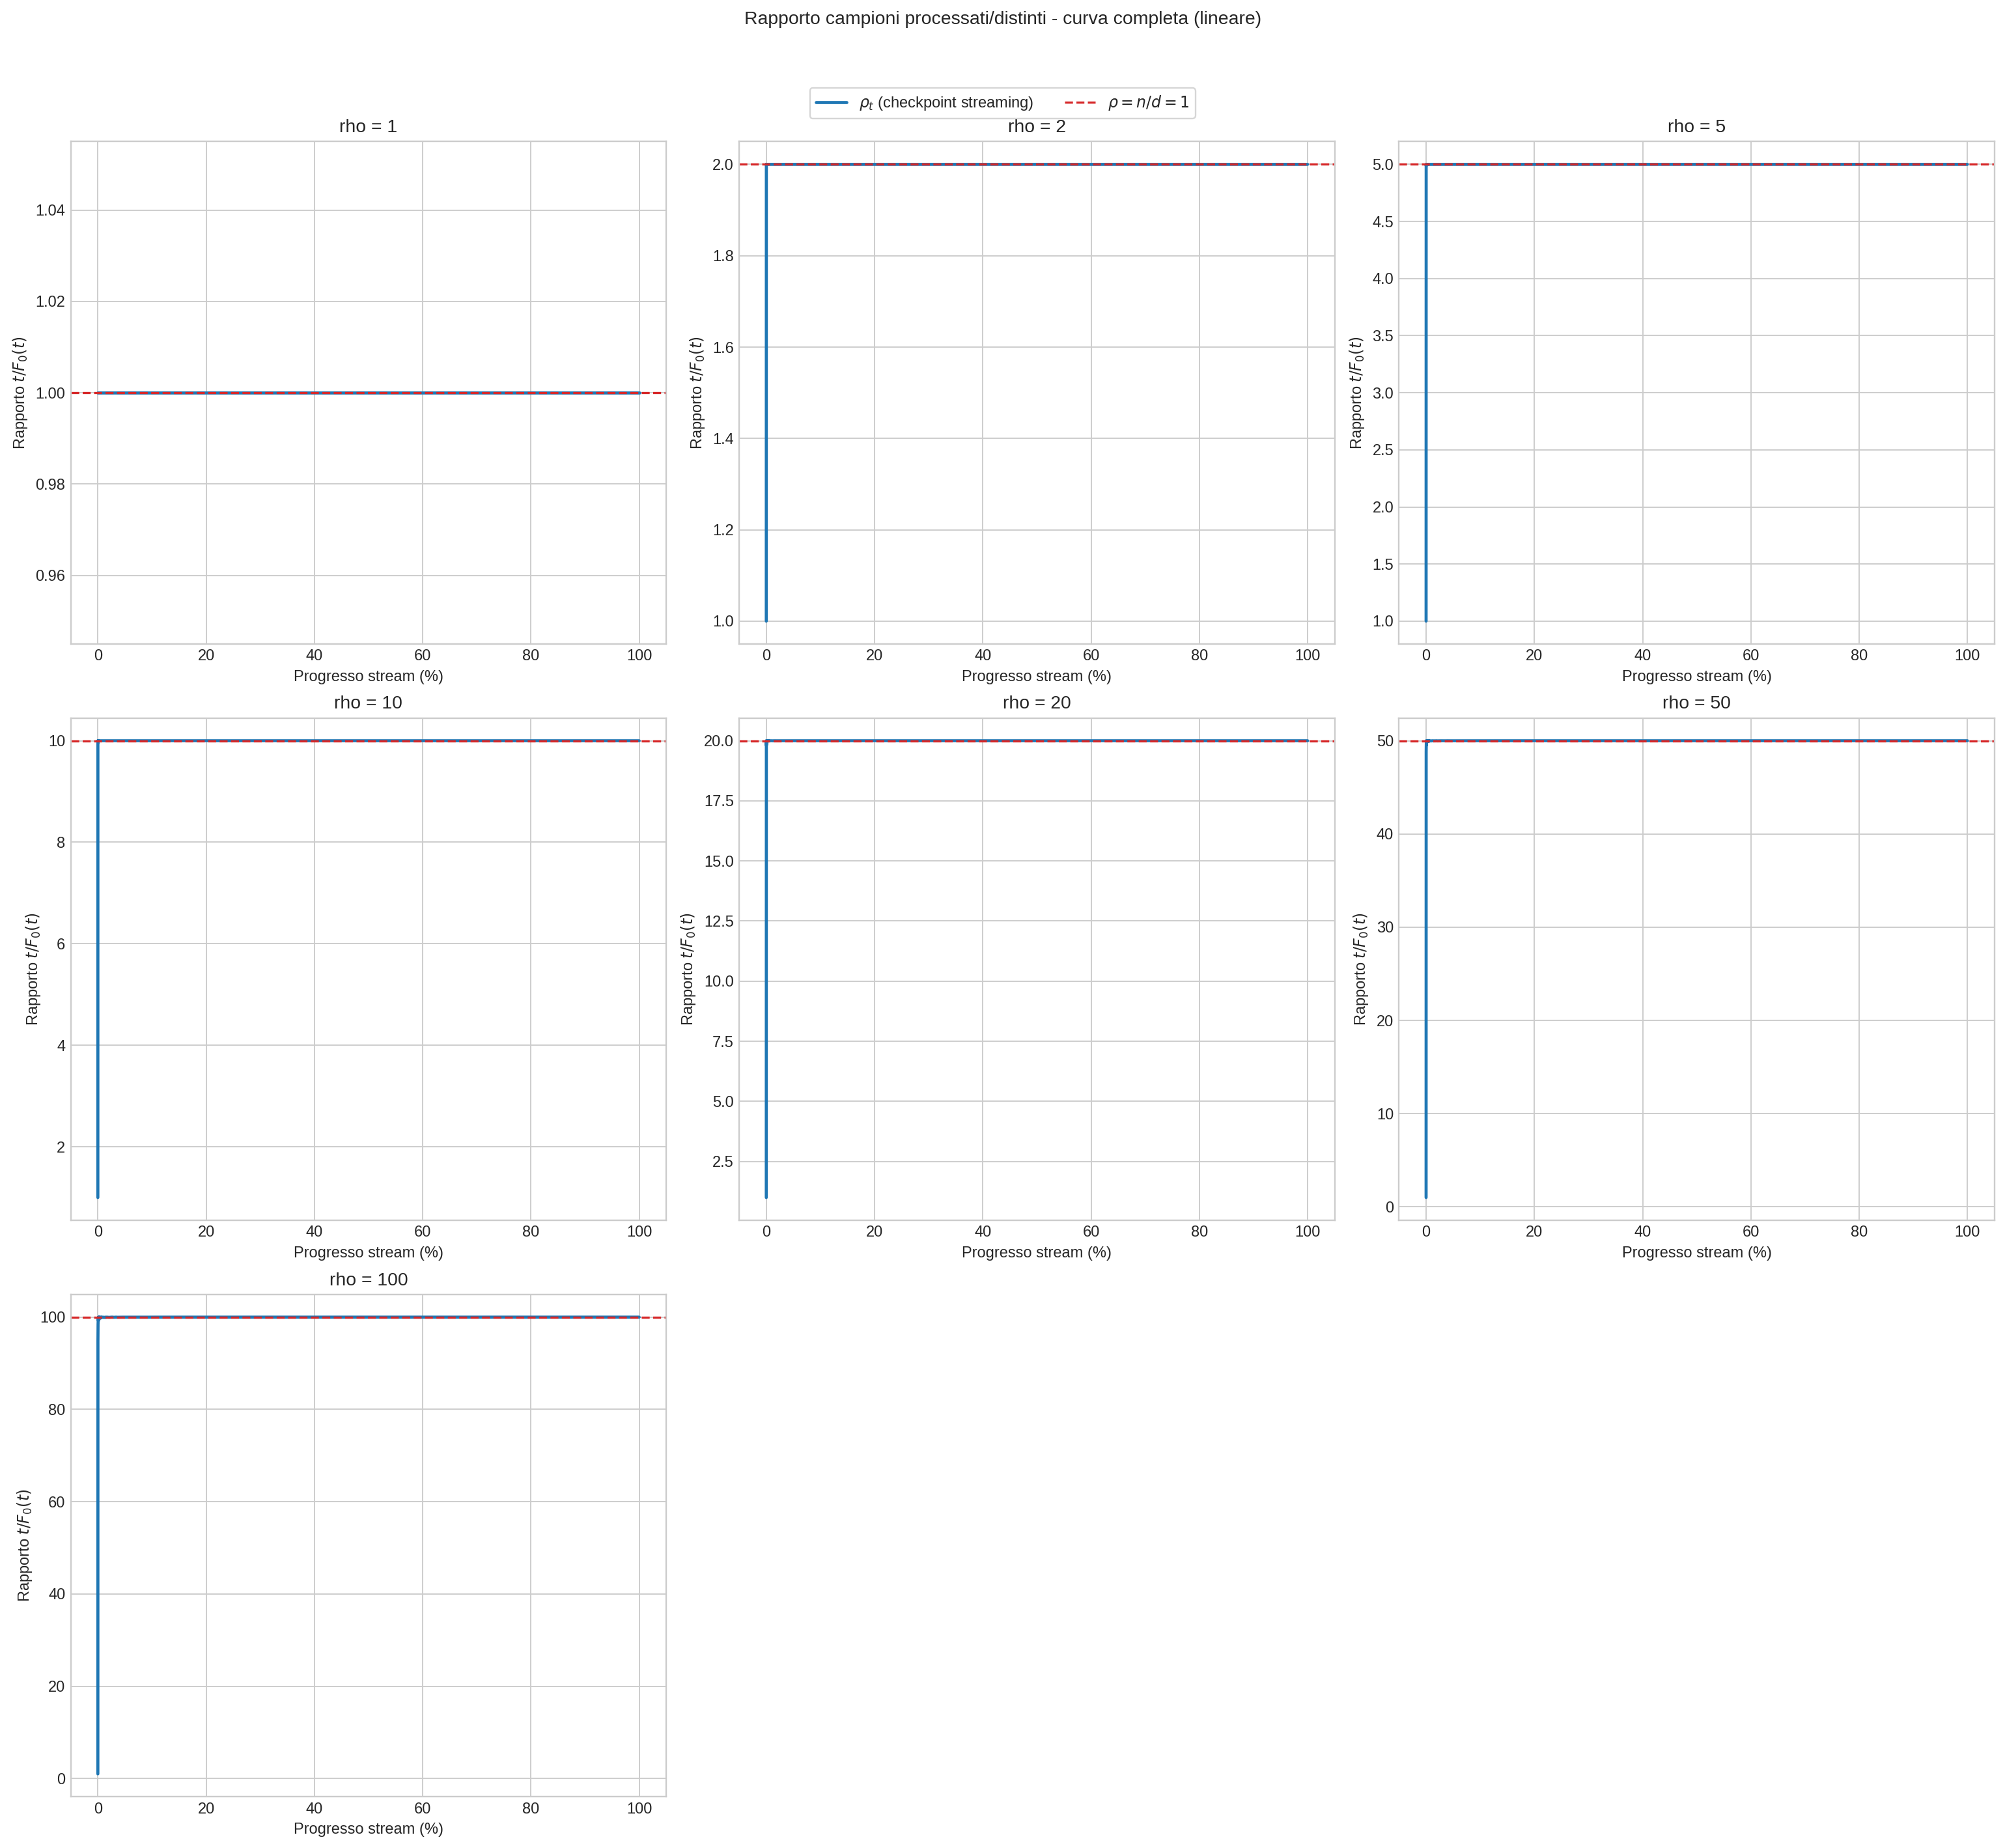
\includegraphics[width=0.96\textwidth]{figures/results/ratio_processed_vs_distinct_streaming_linear.png}
    \caption{Rapporto \(\rho_t=t/F_0(t)\) osservato sui checkpoint di streaming del dataset \texttt{prefix\_constant\_rho}}
    \label{fig:dataset-rho-ratio-linear}
\end{figure}

\begin{figure}[htbp]
    \centering
    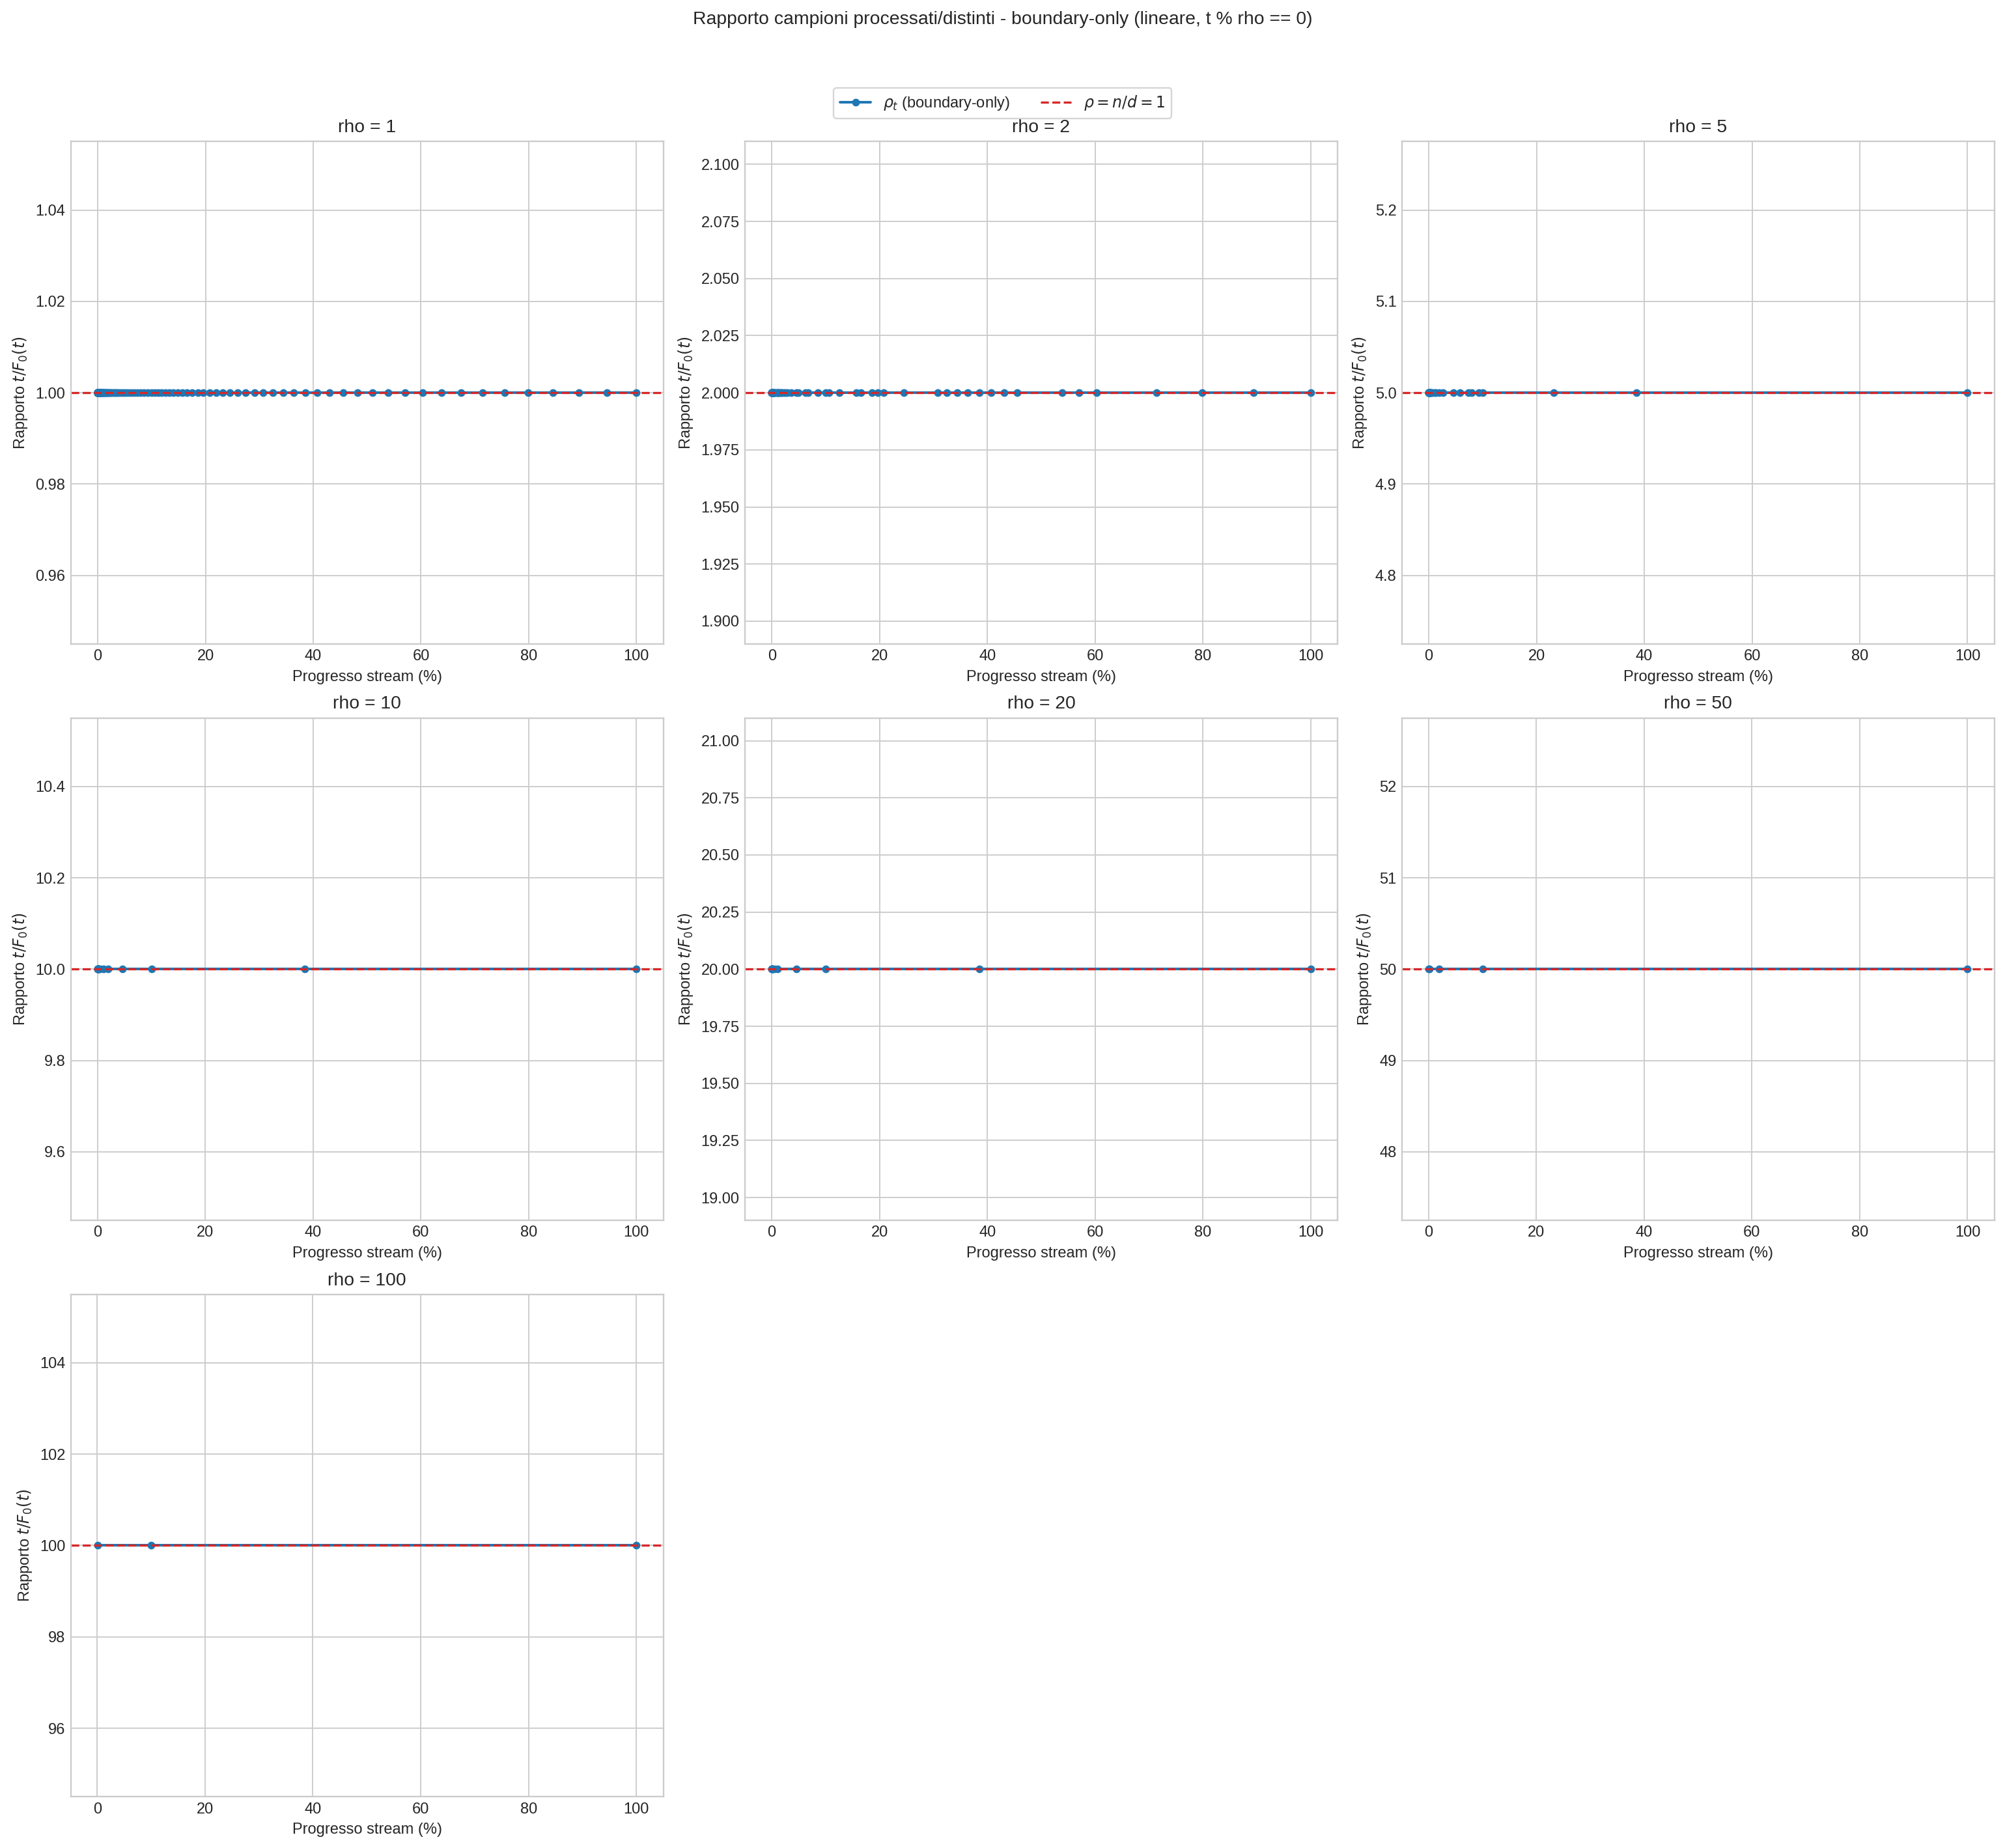
\includegraphics[width=0.96\textwidth]{figures/results/ratio_processed_vs_distinct_streaming_boundary_linear.png}
    \caption{Rapporto \(\rho_t\) osservato ai bordi di blocco, dove per costruzione vale \(\rho_t=\rho\)}
    \label{fig:dataset-rho-ratio-boundary}
\end{figure}

La Figura~\ref{fig:dataset-rho-ratio-linear} mostra la traiettoria completa
osservata ai checkpoint del framework, mentre la
Figura~\ref{fig:dataset-rho-ratio-boundary} evidenzia il comportamento teorico ai
soli multipli di \(\rho\) nei punti di bordo dei blocchi.

\subsection{Riproducibilità del dataset}

La riproducibilità del dataset è garantita da tre elementi:
\begin{itemize}
    \item il seed globale è scritto nell'header del file;
    \item ogni partizione usa un seed derivato in modo deterministico tramite
    \codepath{_derive_partition_seed(seed, partition\_index)};
    \item il generatore è testato esplicitamente in
    \codepath{scripts/tests/test_generate_prefix_constant_rho_dataset.py}.
\end{itemize}

I test verificano la correttezza del formato binario, oltre alla proprietà
\(\sum_t b_t = d\) e alla relazione \(F_0(j\cdot\rho)=j\) insieme alla presenza
di una sola nuova prima occorrenza per blocco e al determinismo del file
prodotto.

\section{Validazione}

La validazione del sistema è distribuita tra test algoritmici, test del
framework e test del generatore del dataset.

\subsection{Test sugli algoritmi}

In \codepath{tests/algorithms} sono presenti test che coprono:
\begin{itemize}
    \item l'accuratezza di base degli algoritmi sui dataset di riferimento;
    \item la validazione dei domini parametrici per HyperLogLog,
    HyperLogLog++ e LogLog;
    \item le proprietà del merge, in particolare commutatività, idempotenza e
    correttezza rispetto al caso omogeneo;
    \item la compatibilità parametrica del merge, con eccezioni esplicite sui
    mismatch non ammessi.
\end{itemize}

Questa parte della validazione è importante perché i limiti di dominio non sono
assunti solo nel testo della tesi, ma difesi direttamente dalle classi concrete.

\subsection{Test del framework}

Il file \codepath{tests/simulation/EvaluationFrameworkTest.cpp} controlla che:
\begin{itemize}
    \item i metadati del framework siano derivati dal dataset e non da valori
    impostati manualmente;
    \item in modalità di flusso il riferimento esatto produca sempre
    \(\hat{F}_0(t)=F_0(t)\) per ogni punto di controllo;
    \item il pianificatore dei punti di controllo copra correttamente il flusso e rispetti il
    budget configurato;
    \item il merge del riferimento esatto coincida con il riferimento seriale;
    \item la serializzazione dei file \texttt{CSV} sia coerente con gli header
    previsti;
    \item il merge eterogeneo copra i casi \texttt{valid},
    \texttt{recoverable} e \texttt{invalid} con le relative strategie.
\end{itemize}

In particolare, i test sul merge eterogeneo verificano quattro regimi:
\begin{itemize}
    \item caso \texttt{valid} con strategia \texttt{direct};
    \item caso \texttt{invalid} con strategia \texttt{reject};
    \item caso \texttt{recoverable} con strategia \texttt{reduce\_then\_merge};
    \item caso \texttt{recoverable} con strategia
    \texttt{unsafe\_naive\_merge}.
\end{itemize}

\subsection{Test del generatore e della catena di esecuzione}

La componente \texttt{Python} è validata da test dedicati sui generatori. In
aggiunta, gli script di orchestrazione costruiscono payload di comandi per la
riga di comando in modo deterministico, fissando namespace dei risultati,
funzioni di hash e griglie parametriche. Anche questa scelta contribuisce alla
riproducibilità complessiva della catena di esecuzione.

\section{Considerazioni progettuali}

La struttura implementativa adottata in questa tesi riflette una scelta precisa:
mettere al centro non un singolo algoritmo, ma la possibilità di confrontare
famiglie algoritmiche diverse in un ambiente coerente.

Dal punto di vista algoritmico, la scelta più importante è l'uso di una
interfaccia comune con validazione rigorosa dei domini e con merge esposto come
operazione di primo livello. Questo rende confrontabili gli sketch non solo in
termini di accuratezza, ma anche in termini di semantica operativa.

Dal punto di vista dell'hashing, la decisione cruciale è stata trattare la
funzione di hash come dipendenza esplicita e non come dettaglio nascosto delle
classi concrete. Questa scelta è ciò che rende possibile, nel capitolo
sperimentale, distinguere in modo netto tra casi omogenei, casi recuperabili e
casi non validi.

Dal punto di vista del framework, la scelta più utile è stata separare dataset,
coordinamento, valutazione e serializzazione. In questo modo gli esperimenti del
capitolo sperimentale non sono stati costruiti come script ad hoc, ma come
istanze diverse della stessa infrastruttura.

Infine, la presenza del dataset \texttt{prefix\_constant\_rho} con bitset di
verità integrato chiude il cerchio metodologico: gli algoritmi sono implementati
come componenti indipendenti, l'hashing è controllabile, il framework li misura
in modo uniforme e il dataset fornisce il riferimento esatto necessario per
leggere correttamente i risultati.
